\chapter{Реализация}
\section{Архитектура}
Ещё на этапе планирования архитектуры приложения было принято решение выделить для логики, связанной с музыкой, отдельный модуль. На данный момент все классы, представляющие собой ключевые музыкальные абстракции (такие как: нота, мелодия, длительность и т.д.), находятся в модуле \textbf{MusicLib}. Во втором модуле (\textbf{App}) содержатся UI-компоненты и некоторые классы, позволяющие связывать пользовательский интерфейс и классы из MusicLib. Благодаря такому разделению появляется возможность гораздо проще проводить тестирование и логически отделять разные абстракции друг от друга.\par
Для представления главных музыкальных абстракций на данный момент существует несколько классов: \textit{Interval}, \textit{NoteRange}, \textit{Melody}, \textit{Note}, \textit{Pause} и \textit{MelodyNote}. Для хранения мелодии применяется класс \textit{Melody}, а для её построения необходима последовательность из нот (\textit{MelodyNote}), либо музыкальных пауз. При этом важным является тот факт, что для представления ноты было принято решение сделать сразу два класса, главное их отличие в том, что \textit{Note} представляет собой просто звук определённой высоты, а \textit{MelodyNote} содержит дополнительные свойства, позволяющие более детально управлять звуком. Классы \textit{NoteRange} и \textit{Interval} представляют собой соответственно диапазон нот (например, для фортепиано) и музыкальный интервал (расстояние между звуками). Кроме этого, существует также множество классов и перечислений для описания различных музыкальных свойств.\par
Модуль App содержит реализацию классов, связывающих описанные выше классы и интерфейс, доступный пользователю. На данный момент реализована возможность создавать свои виртуальные инструменты с помощью наследования от класса \textit{AbstractInstrument} и возможность извлекать из них звуки соответствующих инструментов с помощью \textit{MelodyPlayer}.\par
Было реализованно также и несколько ключевых элементов интерфейса. Например, класс \textit{PianoKeyboard} позволяет отрисовывать на экране клавиатуру переданных размеров и с указанным диапазоном клавиш. Этот элемент полезен как для пользователей, не имеющих реального инструмента, так и для интерфейса некоторых заданий.

\begin{figure}[h!]
  \centering
  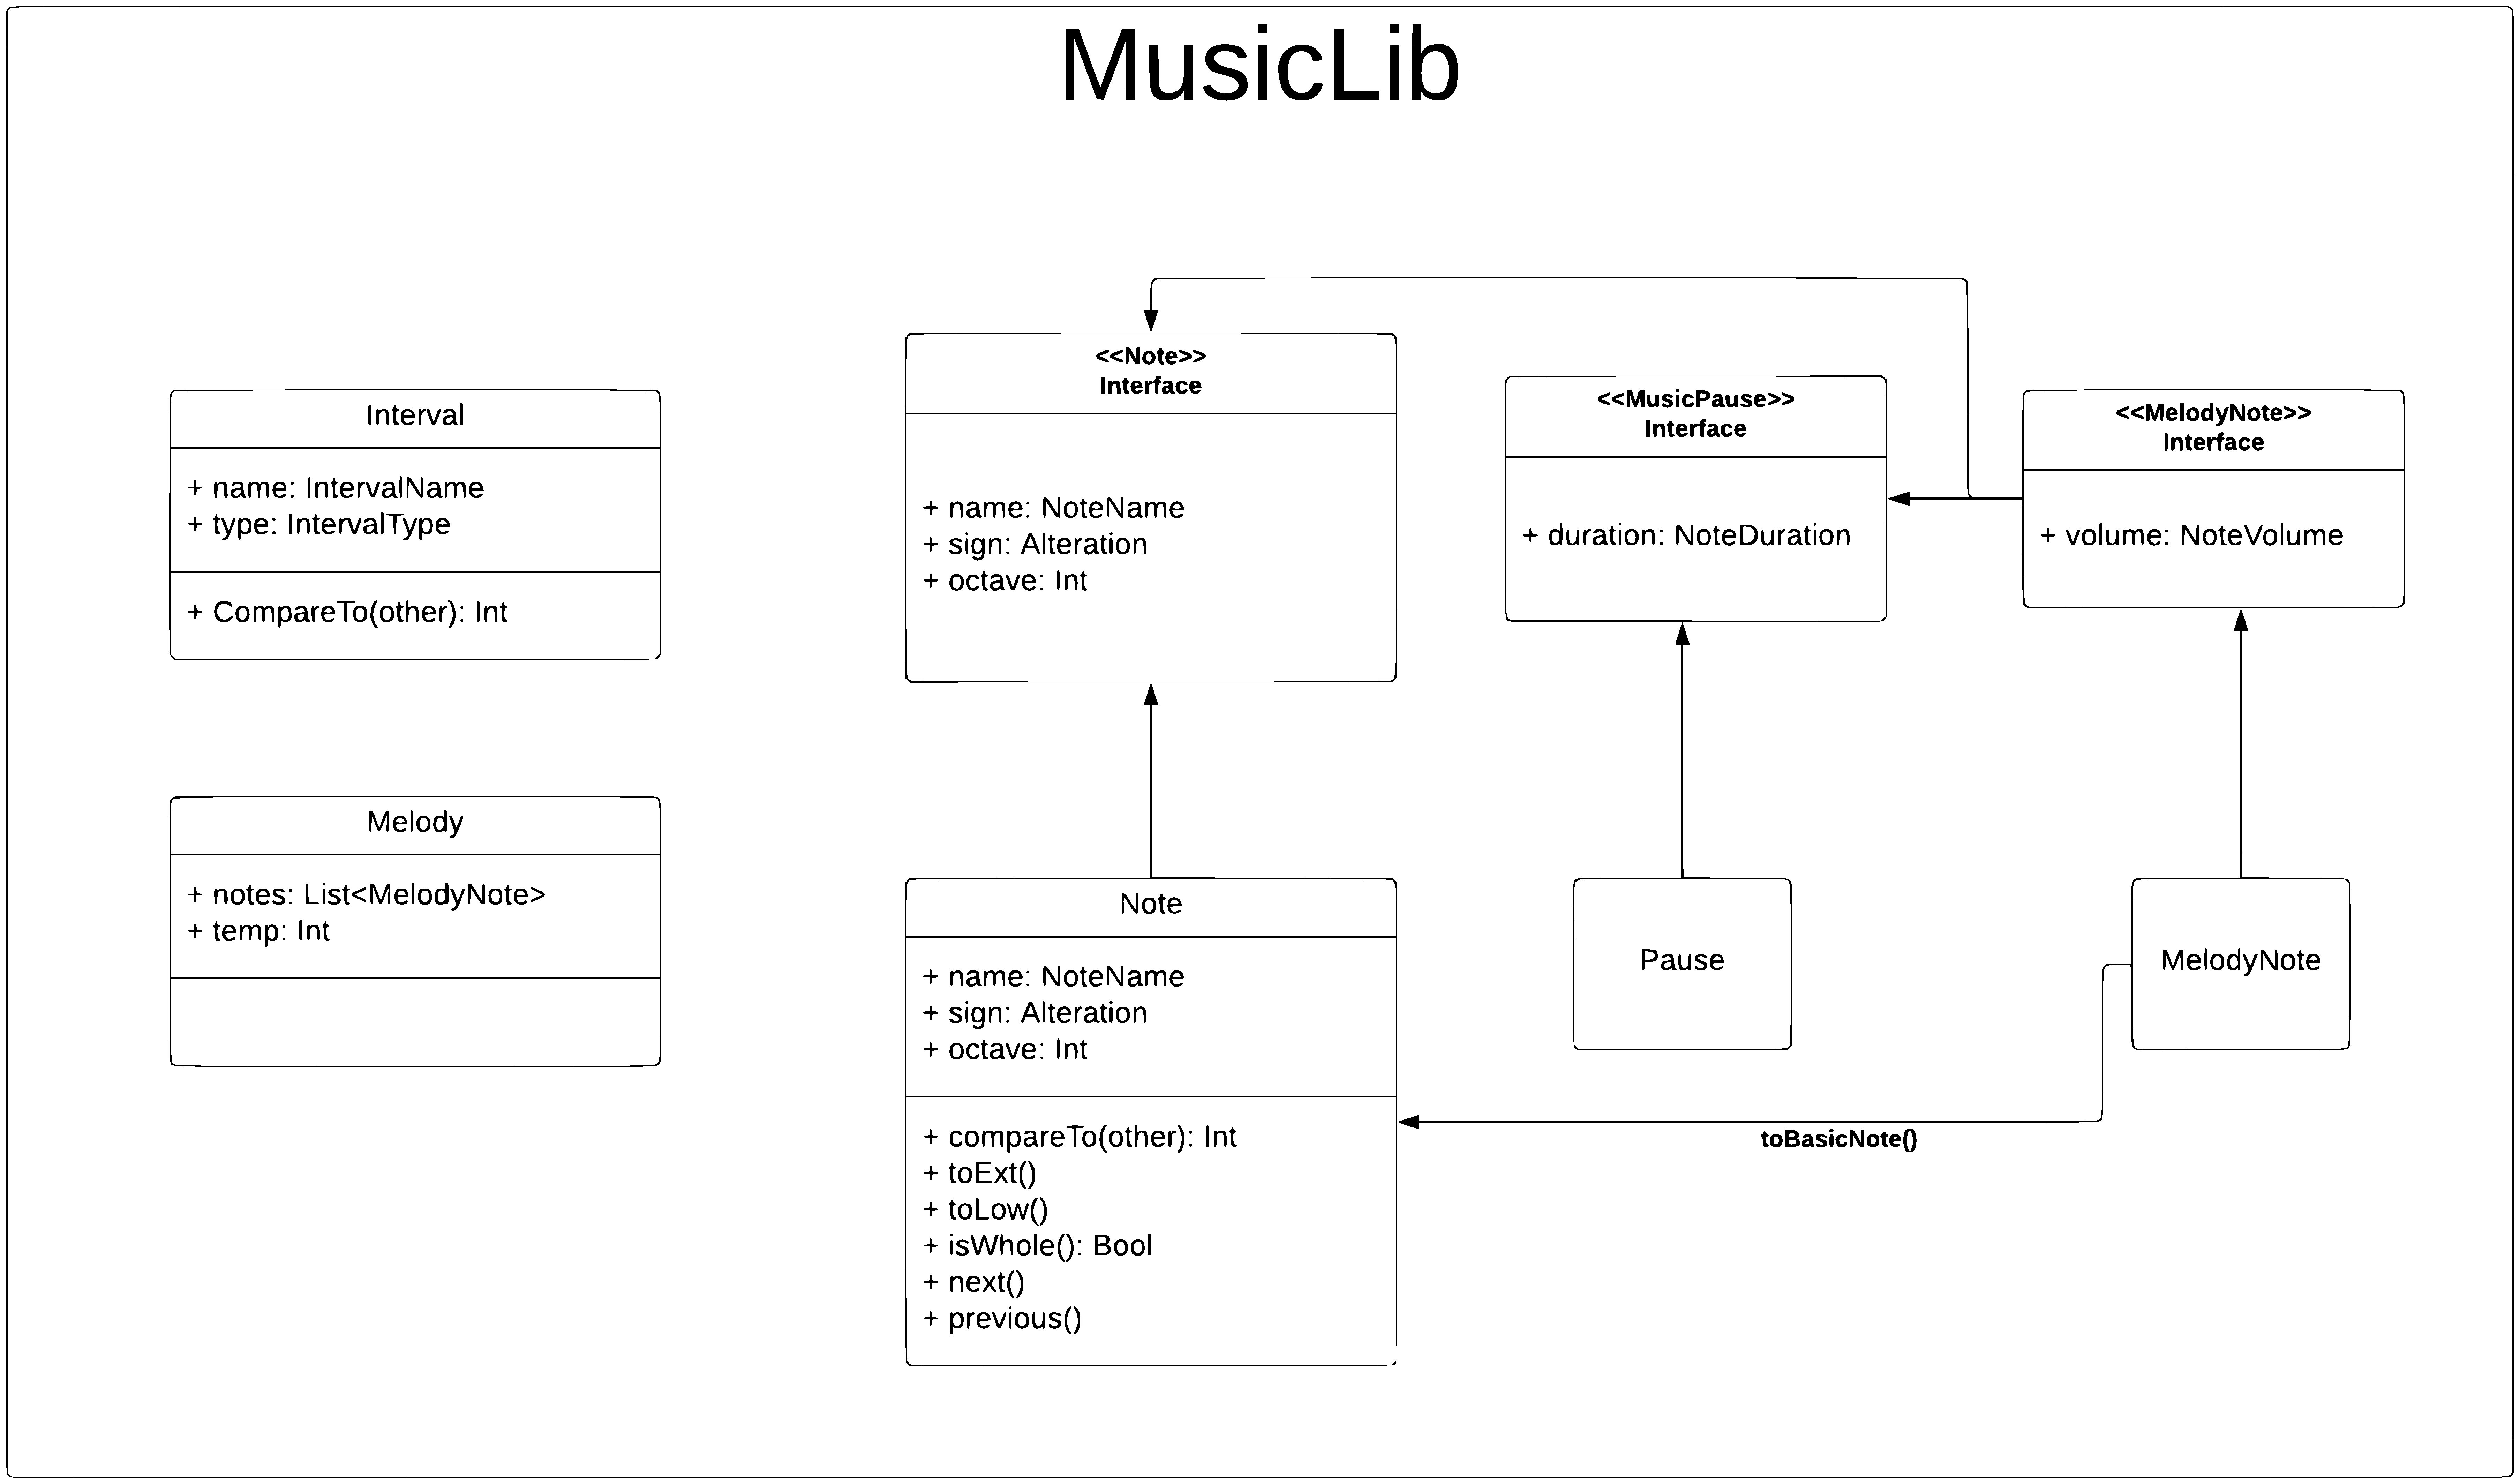
\includegraphics[width=0.55\linewidth]{UML.eps}
  \caption{UML-диаграмма библиотеки.}
  \label{fig:boat1}
\end{figure}
